In diesem Kapitel erfolgt eine Untersuchung des aktuellen Stands der Technik im Bereich der hardwarenahen Softwareentwicklung für Mikrocontroller.
Das Ziel besteht darin, bestehende Ansätze und Konzepte zu analysieren, die das Problem der Treiberauswahl und -abstraktion lösen – insbesondere im Hinblick auf Portabilität und Wiederverwendbarkeit. 
In der vorliegenden Untersuchung wird eine Analyse der gegenwärtig in der Praxis und Forschung eingesetzten Methoden vorgenommen. 
Ziel dieser Analyse ist es, die Übereinstimmung dieser Ansätze mit den Anforderungen der jeweiligen Zielsetzung zu ermitteln und deren Eignung für die Umsetzung einer eigenen Lösung zu evaluieren.

Die Analyse dient zudem der Identifikation möglicher Lücken oder Einschränkungen bestehender Lösungen und trägt somit zur Begründung der Relevanz und Zielsetzung dieser Arbeit bei.


\section{Recherche}
Im Rahmen der Untersuchung wurden sowohl wissenschaftliche Publikationen als auch praxisnahe Quellen herangezogen. 
Zu den praxisnahen Quellen zählen technische Dokumentationen, Open-Source-Projekte und Herstellerdokumentationen.
Der Fokus der Recherche lag auf bestehenden Lösungen für die plattformübergreifende Auswahl von Hardwaretreibern für Mikrocontroller.
Die im Rahmen der Untersuchung verwendeten relevanten Schlüsselbegriffe umfassten unter anderem \textit{Hardware Abstraction Layer, Embedded Driver Portability, CMSIS, Arduino Core, Zephyr RTOS,C++ Hardware API Design}.

Auf diese Weise wurden verschiedene Ansätze zur Hardwareabstraktion und Treiberbereitstellung gefunden.
Die \emph{Common Microcontroller Software Interface Standard} (CMSIS)-Bibliothek ist eine von ARM entwickelte Schnittstelle, die eine weit verbreitete Anwendung findet. 
Sie bietet eine einheitliche Zugriffsebene für Cortex-M-Prozessoren. 
Herstellerbezogene Entwicklungsumgebungen wie die STM32CubeIDE von STMicroelectronics und die Espressif-IDE bieten umfangreiche Hardware-Abstraktionsbibliotheken, die gezielt auf ihre jeweiligen Mikrocontroller-Familien zugeschnitten sind.

Darüber hinaus wurden zwei Open-Source-Projekte auf GitHub analysiert: mcu-cpp und modm. 
Die Zielsetzung beider Ansätze besteht in der Modularisierung der Treiberentwicklung in C++ sowie der Bereitstellung portabler, wiederverwendbarer Hardware-APIs. 
Die Projekte zeigen eine Reihe unterschiedlicher Herangehensweisen in Bezug auf Abstraktionslevel, Architektur und Hardwareunterstützung, was wertvolle Erkenntnisse für die eigene Lösungsentwicklung bietet.
\\
\\
In den folgenden Absätzen werden die einzelnen Plattformen bewertet und potentiellen Vor- und Nachteile benannt; auch in Bezug auf die Anforderungen der eigenen Lösung. 
%Wie machen das andere; auch in Form kommerzieller Werkzeuge (cubeIDE, Espressif):
%\begin{itemize}
% 	\item CMSIS
%	\item Espressif IDE
%\end{itemize}

\section{Bewertung der Alternativlösungen}
\subsection{STM32Cube}
Die STM32Cube-Umgebung der Firma STMicroelectronics bietet ein gesamtes System, von der Auswahl und der Konfiguration der Hardware bis hin zu einer IDE zur Softwareentwicklung und einer Software um den internen Speicher der MCUs zu programmieren.
Aufgeteilt auf:
\paragraph{STMCUFinder}
	um die Hardware zu finden, die den notwendigen Anforderungen gerecht werden kann.
	Dafür gibt es die Möglichkeit, mit verschiedenen Filtern die Auswahl derart einzuschränken, dass nur noch die passenden Mikrokontroller übrig bleiben.
	Diesen Schritt kann man nicht nur allein für die MCUs und MPUs machen, sondern auch für gesamte Hardwareboards.
	Hier kommen Filter hinzu, welche Funktionen die Hardware bereits integriert hat.
	Ist die passende Hardware ausgewählt, kann aus dieser Übersicht direkt der STM32CubeMX gestartet werden.

\paragraph{STM32CubeMX} 
	zur Konfiguration der Hardware, d.h. Benennung und Funktionszuweisung der Pins, Aktivieren oder Deaktivieren von Registern und Protokollen, Konfiguration der internen Frequenzen. 
	Nach der Konfiguration kann der Code für das Projekt generiert werden.
	In diesem Schritt werden die notwendigen Pakete, Treiber (HAL, CMSIS) und Firmware für die ausgewählte Hardware geladen.

\paragraph{STM32CubeIDE}
	um Anwendungen und Software für die MCUs zu entwickeln und implementieren.
	Die Entwicklungsumgebung, basierend auf Eclipse, bietet neben dem Codeeditor ein eigenes Buildsystem, das mit Make und der \texttt{arm-none-ebai-gcc}-Toolchain arbeitet und einen Debugger hat, mit dem nicht nur Code sondern auch das Verhalten der Hardware beobachtet werden kann um Fehler zu erkennen.
\\
\\
Hier ist Positiv hervorzuheben, dass sehr viel über eine Benutzeroberfläche eingerichtet werden kann, was den Einstieg in die Embedded-Entwicklung etwas leichter gestaltet.
Durch das große Portfolio an an MCUs und Hardwareboards, die alle mit der STM32Cube-Umgebung kompatibel sind, ist es nicht direkt notwendig andere Optionen in betracht zu ziehen. 
Allerdings ist das auch ein Aspekt, der bedacht werden muss. 
Das Softwarepaket funktioniert nur mit der STM32-Hardware.
Der Einsatz mit MCUs anderer Hersteller ist damit nicht vorgesehen.

Für allgemeine Projekte bzw. st-fremde Hardware besteht die Möglichkeit, in der STM32CubeIDE leere CMake-Projekte zu erstellen.
Hier müssen dann die benötigten Pakete und Treiber selber inkludiert werden.
Ein Buildsystem müsste selber eingebunden und mit eigenen CMake-Dateien implementiert werden.


% TODO: chap5 Espressif-IDE
%\subsection{Espressif-IDE}


\subsection{mcu-cpp}
% TODO: chap5 mcu-cpp: Quellen-Verlinkung
Das Open-Source-Projekt \emph{mcu-cpp} verwendet einen eigenen \texttt{namespace} um die einzelnen Funktionen und Klassen zu gruppieren.
\emph{Namespaces} sind eine Möglichkeit in C++ um Variablen, Klasse und Funktionen zu gruppieren, damit Konflikte bei der Benennung solcher Identifizierer zu vermeiden.
Die ermöglicht einen sauber-strukturierten und lesbaren Applikationscode zu schreiben, in dem man nachvollziehen kann, wer was aufruft.
Basierend auf den virtuellen Klassen, implementieren die jeweiligen MCUs die Methoden damit diese für sich funktionieren.
Um innerhalb einer Produktfamilie, z.B. STM32F0 MCUs, die richtigen bzw. alle notwendigen Ports zu aktivieren, gibt es eine zusätzliche Datei \texttt{gpio\_hw\_mapping.hpp}.
In dieser werden einzelne Ports, die nicht auf jeder MCU verfügbar sind, durch bedingte Kompilierung aktiviert oder nicht.
Die Information, welche Hardware verwendet wird, muss entweder in der \texttt{CMakeLists.txt} oder im Code mit \texttt{\#define} angegeben sein.
Zusätzlich werden die CMSIS-Treiber verwendet, die die Startdateien bereit stellen.
Als RTOS wird aktuell FreeRTOS verwendet.
%Dies ermöglicht
Allerdings fehlen hier die offizielle \emph{Hardware-Abstracition-Layer} (HAL), die bereits vorgefertigte Strukturen und Funktionen für die einzeln Hardwarefunktionen implementiert haben.
Stattdessen werden diese durch die Implementierung der virtuellen Klassen ersetzt.
Das sorgt im weiteren Verlauf dafür, dass die Funktionen auf Basis der virtuellen Klassen für jede neue MCU-Familie neu implementiert werden muss, was einen für wiederholten Aufwand sorgt und den Anforderungen an die Lösung widerspricht.



\subsection{modm}
% TODO: chap5 modm: Quellen-Verlinkungß
Das Open-Source-Projekt \emph{modm} dient als Baukasten um zugeschnittene und anpassbare Bibliotheken für Mikrocontroller zu generieren.
Dadurch ist es möglich, dass eine Bibliothek nur aus den Teilen besteht, die tatsächlich in der Applikation und im Code verwendet werden müssen, ohne das es einen unnötig großen Overhead gibt.
Um das zu bewerkstelligen wird eine Kombination aus \texttt{Jinja2}-Template-Dateien, \texttt{lbuild}-Pyhton-Skripte und eigenen Moduldefinitionen verwendet, mit der der Code für die Bibliotheken generiert wird.
Die Templatedateien enthalten Platzhalter.
Die Werte kommen aus \texttt{YAML} und \texttt{JSON}-Dateien, die von den \texttt{lbuild}-Pyhtonskripten gelesen und in die entsprechenden Positionen der Platzhalter, während des Buildprozesses, eingefügt werden.
 
Um eine Bibliothek zu erstellen, muss ein Prozess über die Konsole gestartet werden.
modm hat bereits vordefinierten Konfigurationen für eine große Auswahl an MCUs.
Mit diesen kann die Bibliothek für ein Projekt erstellt/gebuildet werden.

Will man aber Module verwenden, die in der vordefinierten Konfiguration nicht enthalt sind, kann man Module einzeln zu der \texttt{project.xml} hinzufügen.
Um sehen zu können welche Module zur Verfügung stehen muss folgende Zeile in der Konsole ausgeführt werden:

\vspace{3mm}
\begin{lstlisting}[language=bash, caption={Konsolenbefehl um verf\"ugbare Module aufgelistet zu bekommen; hier f\"ur den STM32C031C6T6 Mikrokontroller.}, label={lst:modm_lbild_discover}]
\modm\app\project>
	lbuild --option modm:target=stm32c031c6t6 discover
\end{lstlisting}

Sobald die gewünschten Module hinzugefügt wurde, beginnt der Installations- bzw. der Generierungsprozess der Library. 
Gibt man nun \texttt{lbuild builld} in der Konsole ein wenn man sich im \texttt{app/project}-Verzeichnis kann die Bibliothek erstellt werden.
Nach erfolgreichem Build erscheint in dem Projektverzeichnis ein neuer Ordner \emph{modm}.
Dieser enthält die generierten Dateien der ausgewählten Module.

Positiv hervorzuheben ist hier das (vordergründige) simple Hinzufügen von Modulen.
Da das Projekt aktuell bereits sehr umfangreich ist und sehr viele Mikrokontroller und Optionen unterstützt, bietet es eine große Auswahl an Modulen, die beliebig zu einem Projekt hinzugefügt werden können.

Allerdings ist zu beachten, dass falls man zukünftig neue Module oder Mikrokontroller hinzufügen will, müssen diese an die bestehende Struktur angepasst und in das Zusammenspiel von Python, Jinja2 und den YAML/JSON-Dateien integriert werden.
Dies ist mit einem sehr hohen Aufwand verbunden.


%%%%%%%%%%%%%%%%%%%%%%%%%%%%%%%%%%%%%%%%%%%%%%%%%%%%%%%%%%%%%%%%%%%%
% Notizen
%%%%%%%%%%%%%%%%%%%%%%%%%%%%%%%%%%%%%%%%%%%%%%%%%%%%%%%%%%%%%%%%%%%%
\section{Notizen}
Ähnlich zu dem Projekt mcu-cpp soll die eigene Lösung auch Interfaces bzw. virtuelle Klassen als Basis verwenden, die dann von allen MCUs abstrahiert werden können.
Auf diese Weise bekommt jede MCU eine eigene Kindklasse, über die die richtigen Treiber ausgewählt werden.



\begin{itemize}
	\item Interface/virtuelle Klassen als Basis
	\item \textbf{Factory Methode} zur Erzeugung der Objekte $\rightarrow$ Entwurf der Architektur
	\item [$\Rightarrow$] Adapter implementieren um andere MCUs verwenden.
	\item [$\Rightarrow$] Was muss alles bedacht werden:
	\begin{itemize}
		\item Pin Initialisierung $\rightarrow$ STM32 ok; wie bei anderen MCUs?
		\item Interrupt-Handling
		\item 
		\item Flashen des Chips mit dem Programm
	\end{itemize}
	\item einfache Make commands rufen CMake build commands auf
	\item Ninja als Generator $\rightarrow$ wird von ESP, mcu-cpp, Zephyr schon benutzt. STM32 nutzt make, kann aber getauscht/angepasst/konfiguriert werden
	\item Treiber (HAL, vllt. CMSIS) als Submodule
\end{itemize}

\subsection{Architektur}
\subsubsection*{Factory}
\begin{itemize}
	\item erstellt und returned Hardware-Instanz
	\item für HW-Inistialisierung
	\item erstellt Instanz je nach Hardware $\rightarrow$ \texttt{\#ifdef}
\end{itemize}

\subsubsection*{Gpio}
\begin{itemize}
	\item eigen Klasse
	\item erstmal für STM32 $\rightarrow$ danach Adapter für andere?
\end{itemize}

Keine \texttt{setter}
\begin{itemize}
	\item Pin wird nur einmal initialisiert
	\item normalerweise keine nachträgliche Änderungen zur Laufzeit
\end{itemize}

%%%%%%%%%%%%%%%%%%%%%%%%%%%%%%%%%%%%%%%%%%%%%%%%%%%%%%%%%%%%%%%%%%%%
% PROBLEME
%%%%%%%%%%%%%%%%%%%%%%%%%%%%%%%%%%%%%%%%%%%%%%%%%%%%%%%%%%%%%%%%%%%%
\subsection*{Probleme:}
\begin{itemize}
	\item Interruptfunktionen $\rightarrow$ werden automatische aufgerufen und nicht vom Entwickler. Wenn ein Interrupt auftritt wird der Rest der HAL \& der MCU informiert.\\ \textbf{Frage:} Wie kann es umgesetzt werden, dass das GPIO-Objekt der API und der Code der Anwendungsschicht aus der HAL und den Registern über einen Interrupt informiert werden?
	\item \texttt{\_\_HAL\_RCC\_GPIOA\_CLK\_ENABLE()} setzt den Pin im Inputregister IDR $\rightarrow$ ID14.
	
\end{itemize}

\subsection*{Gelöst}
\begin{itemize}
	\item GPIO init $\rightarrow$ MX\_GPIO\_Init() startet mit \texttt{iocurrent} bei $0$. Mit dem Aufruf durch das Objekt startet \texttt{iocurrent} auf etwas extrem Hohen. \\ $\Longrightarrow$ Ist Egal. \texttt{iocurrent} bekommt direkt einen richtigen Startwert zugewiesen.
	\item Statt \texttt{ID15} für Pin 15 zu wechseln, werden die \texttt{ID0-3} gewechselt. Diese ersten $4$ Pin ergeben binär auch $15\ =\ 1111\ =\ 1*2^3\ +\ 1*2^2\ +\ 1*2^1\ +\ 1*2^0$ \\ \textbf{Lösung:} Nicht den Wert $15$ dem Pin Attribut geben sondern am Bit $15$, dass diese Bit dann auf $1$ gesetzt wird.
	\item Wenn die LED an ist, d.h. wenn der Pin gesetzt ist, verändert sich der Pin des Tasters, ohne dass dieser betätigt wurde. Wieso?\\ \textbf{Beobachtung:} Ob bei \texttt{readPin()} Register ID$14$ oder ID$9$ verwendet wird (es sollte $9$ sein; $14$ ist nur im Debugger aktiv und für uns uninteressant) schon zufällig zu sein.\\ \textbf{Lösung:} Mit Pin-Debouncing und Implementierung einer Timer-Klasse konnte das zufällige Verhalten gelöst werden. 
	\item Mit \texttt{time.hpp} und \texttt{stm32::Gpio::Pull::Up} funktioniert die Schaltung.\\ \textbf{Frage:} Wieso funktioniert das mit \texttt{Pull::Up} und nicht mit \texttt{Pull::None} od. \texttt{Pull::Down}?\\ \textbf{Antwort:} Mit \texttt{Pull::None} befindet sich der Schalter in einem \emph{float} Zustand. In diesem werden besonders Einflüsse der Umwelt, sog. Noise/Rauschen aufgenommen, die das Verhalten der Schaltung unberechenbar machen. Dieses zufällige Verhalten sollte vermieden werden, besonders in einem sicherheitskritischen Umfeld.
\end{itemize}

\subsection*{Fragen wegen der Implementierung:}
\begin{itemize}
	\item 
\end{itemize}

\vspace{3mm}

mapping $\rightarrow$ stm32c0xx.h $\rightarrow$ stm32c031xx.h mit allen TypeDefs $\rightarrow$ system\_stm32c031xx.h

$\Longrightarrow$ include Fehler: statt nur stm32\_hal\_gpio.h, besser stm32\_hal.h einbinden.
\\

Verwendung von STM32CubeIDE für bessere Übersicht beim Debuggen über die Register.
\\

\vspace{3mm}
\begin{figure}[H]
	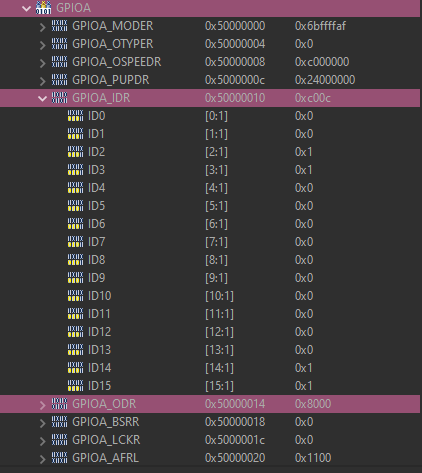
\includegraphics[width=\textwidth]{stm32_c031c6_clean_registers_setPin.PNG}
	\caption{Register beim setzen des Pin.}
	\label{fig:stm32_register_setPin}
\end{figure}

\vspace{3mm}
\begin{figure}[H]
	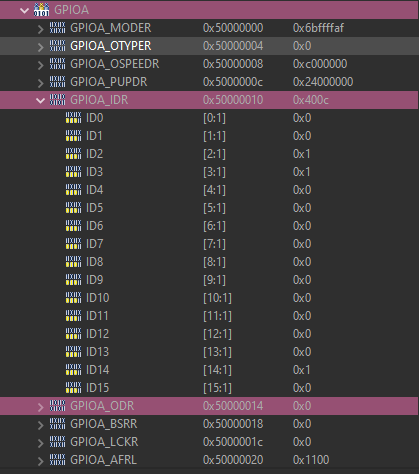
\includegraphics[width=\textwidth]{stm32_c031c6_clean_registers_resetPin.PNG}
	\caption{Register beim zurücksetzen des Pin.}
	\label{fig:stm32_register_resetPin}
\end{figure}

In den Abbildungen \autoref{fig:stm32_register_setPin} und \autoref{fig:stm32_register_resetPin} ist der Wert von Pin 15 (ID15 \& OD15) zu beobachten. Bei \texttt{0x0} wird der Pin zurückgesetzt und die LED leuchtet nicht mehr. Bei \texttt{0x1} wird der Wert auf $1$ gesetzt und die LED beginnt zu leuchten.

Die Funktionen \texttt{HAL\_GPIO\_WritePin(GPIO\_TypeDef \*GPIOx, uint16\_t GPIO\_Pin, GPIO\_PinState PinState)} steuern nicht die in \autoref{fig:stm32_register_setPin} und \autoref{fig:stm32_register_resetPin} gezeigten Register IDR und ODR an, sondern die Set- und Reset-Register BSRR und BRR. 

Diese Register sind \emph{write only}, d.h. sie können nicht ausgelesen werden.
Wird die Funktion korrekt ausgeführt, kann dass Verhalten an den Registern IDR und ODR beobachtet werden.



























